
This section presents the results of the evaluation and answers the research questions.

% Due to space constraints, we report our results at the project level and provide examples at the class level. Full results are available in our replication package.\footnote{The link will be provided in next version}

\subsection{Coupled branches coverage by \cling (RQ1.1)}

% \begin{figure}[t]
%     \centering
%     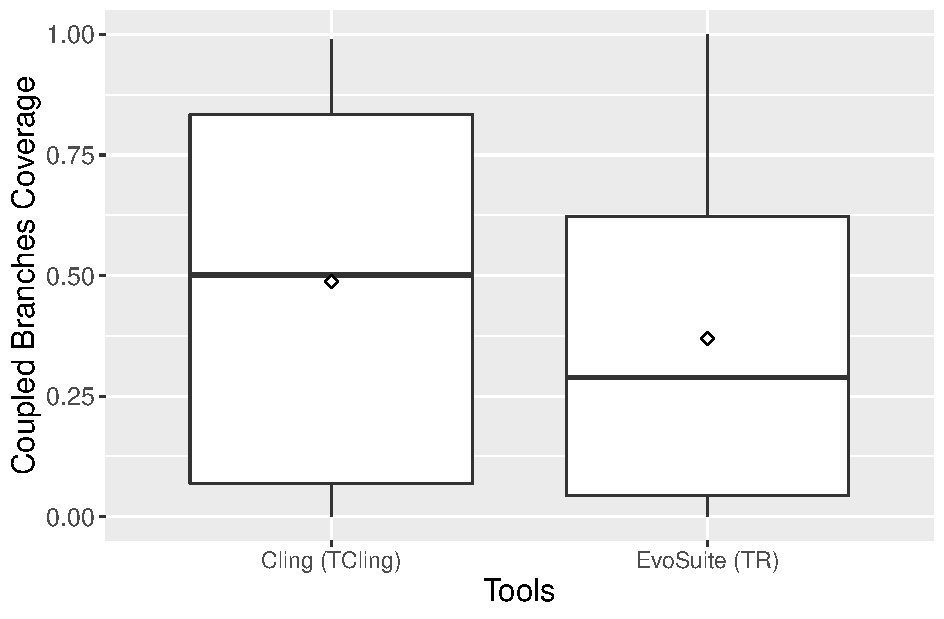
\includegraphics[width=0.48\textwidth]{figures/cbc-total.pdf}
%     \caption{Total coupled branches coverage of $T_{\cling}$ and $T_R$.}
%     \label{fig:cbccoverage:total}
% \end{figure}
    

\begin{figure}[t]
    \centering
    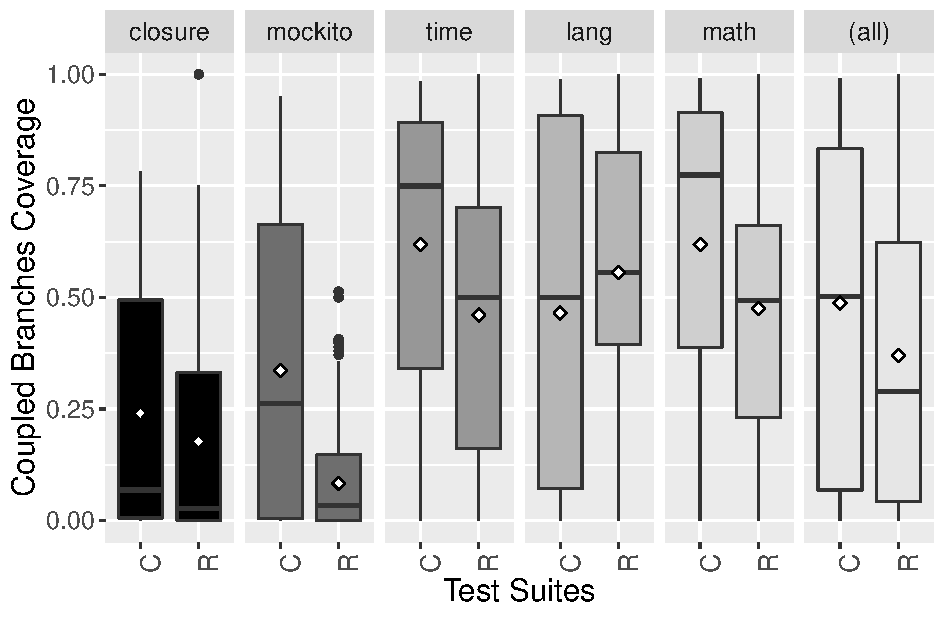
\includegraphics[width=0.75\textwidth]{papers/cling/figures/cbc-per-project.pdf}
    \caption{Total coupled branches coverage achieved by $T_{\cling}$ (C) and $T_R$(R). ($\diamond$) denotes the arithmetic mean and (---) is the median.}
    \label{fig:cbccoverage}
\end{figure}

\begin{figure}[t]
    \centering
    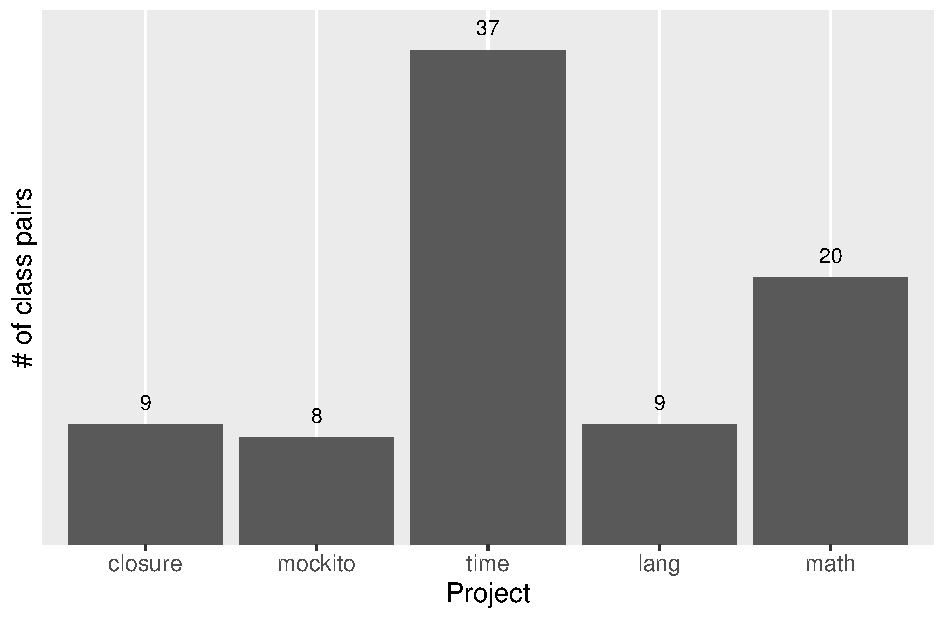
\includegraphics[width=0.75\textwidth]{papers/cling/figures/cbc-higher-than-50.pdf}
    \caption{Number of class pairs, in which \cling achieves a coupled branch coverage higher than 50\%}
    \label{fig:cbchigher50}
\end{figure}


As reported in Table \ref{tab:cling:projects}, \cling did not identify any coupled branches for four pairs of classes (one in \texttt{mockito} and three in \texttt{time}). This is due to the absence of target branches in either the caller or the callee. 
Those four couples have been excluded from the results presented in this section.

Figure \ref{fig:cbccoverage} presents the coupled branches coverage of the $T_{\cling}$ in all of the projects. On average (the diamonds in Figure~\ref{fig:cbccoverage}), the test suites generated by \cling cover 49\% of coupled branches.
For 83 out of 140 (59.2\%) of the pairs, \cling can generate test suites achieving a coupled branches coverage above 50\%. 

The most covered couples are in the \texttt{math} project ($\overline{CBC_C}=61.9\%$), followed by \texttt{time} ($\overline{CBC_C}=61.8\%$) and \texttt{lang} ($\overline{CBC_C}=46.5\%$). The least covered couples are in the \texttt{closure} ($\overline{CBC_C}=24\%$)  and \texttt{mockito} projects ($\overline{CBC_C}=33.6\%$), which are also the projects with the highest number of coupled branches in Table~\ref{tab:cling:projects} (10,542 coupled branches on average for all the class pairs in \texttt{closure} and 1,185 coupled branches on average in \texttt{mockito}).

In total, \cling could generate at least one test suite achieving a coupled branches coverage higher than 50\% for 83 out of 140 pairs (depicted in Figure \ref{fig:cbchigher50}).

For 9 caller-callee pairs, \cling could not generate a test suite able to cover at least one coupled branch out of 20 executions: 3 for \texttt{math} and \texttt{mockito}, 2 for \texttt{closure}, and 1 for \texttt{lang} (with \texttt{StringUtils} as callee class, misleading the search process). The other 8 pairs cannot be explained solely by the complexities of the caller (with a cyclomatic complexity ranging from 8 to 5,034 for those classes) and the callee (with a cyclomatic complexity ranging from 1 to 2,186) or the number of call sites (ranging from 1 to 177). This calls for a deeper understanding of the interactions between caller and callee around the call sites. In our future work, we plan to refine the caller-callee pair selection (for which we currently looked at the global complexity of the classes) to investigate the local complexity of the classes around the call sites.

\subsubsection{Summary}
On average, the generated tests by \cling cover 49\% of coupled branches.
In  83 out of 140 (59.2\%) of the pairs, these test suites achieve a CBC higher than 50\%.
\subsection{CBC achieved by \cling vs. \evosuite (RQ1.2)}
For this research, since $T_E$ covers only branches in the callee class (\ie it does not call any methods in the caller class), the coupled branches coverages achieved by these tests are always zero. 
Hence, for this research question, we compare the tests generated by \cling ($T_{\cling}$) against the tests generated by \evosuite applied to the caller class ($T_R$) in terms of coupled branches coverage. 

Figure \ref{fig:cbccoverage} presents the coupled branches coverage of the $T_{\cling}$ and $T_{R}$ in all of the projects. As we expected, the number of covered coupled branches by $T_{\cling}$ is higher than $T_{R}$ in total (right-side boxplots in Figure~\ref{fig:cbccoverage}). On average (the diamonds in Figure~\ref{fig:cbccoverage}), the test suites generated by \cling cover 13\% more coupled branches (in percentage points) compared to 36\% for the average coupled branches coverage performed by $T_{R}$.


In general $T_{\cling}$ achieves a higher CBC compared to $T_{R}$. On average, the coupled branches coverage achieved by $T_{R}$ is lower than \cling in all of the projects except \texttt{lang}. The average coupled branches coverage of \evosuite in this project is $55.6\%$. We have manually analyzed the search progress of \cling  for pairs of classes where the number of covered coupled branches is low (\ie lower than 10). 

We noticed that \cling is counter-productive for specific class pairs where the callee class is \texttt{StringUtils}. In those cases, the initially generated test cases by \cling throw a \texttt{NoSuchFieldError} in the callee class (\texttt{StringUtils} here). Nevertheless, since these test cases achieve small approach levels and branch distances from the callee branches, their fitness function is lower than the other test cases. Since \cling tries to minimize the search objectives, these test cases are selected for the next generation. However, these tests are not solutions that can cover the coupled branches. Therefore, the small fitness function for these solutions drives the search process in local optima and misguides the search process.
 

\subsubsection{Summary}
On average, the generated test suites by \cling cover 13\% more coupled branches compared to \evosuite. 

\subsection{Comparison of Mutation Scores (RQ2)}
 
 
\begin{figure}[t]
    \centering
    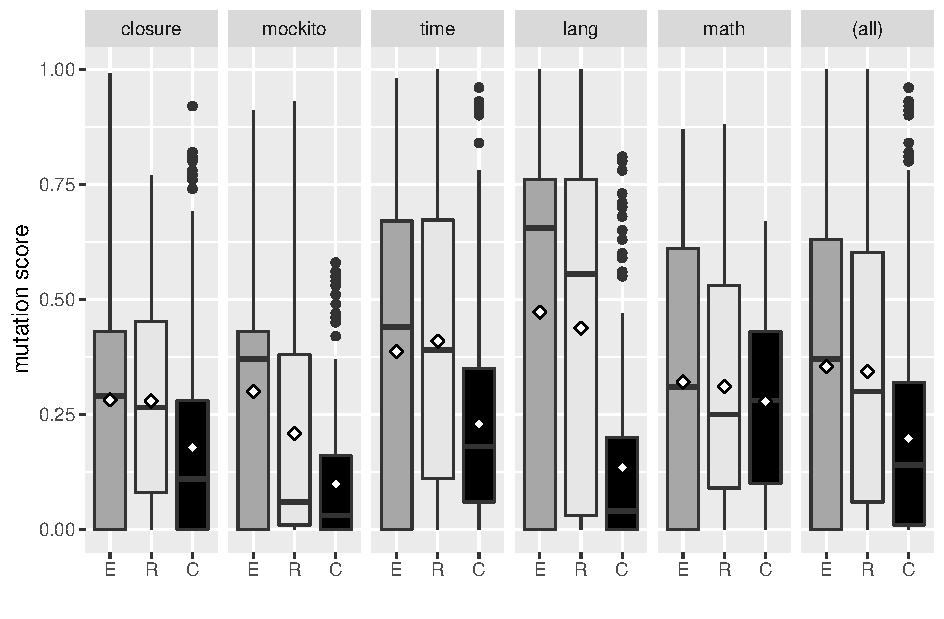
\includegraphics[width=0.75\textwidth]{papers/cling/figures/mutation-coverage-boxplot.pdf}
    \caption{Mutation score for $T_E$, $T_R$, and $T_\integration$ when mutating $E$. ($\diamond$) denotes the arithmetic mean and (---) is the median.}
    \label{fig:mutation:boxplot}
\end{figure}

\begin{figure}[t]
    \centering
    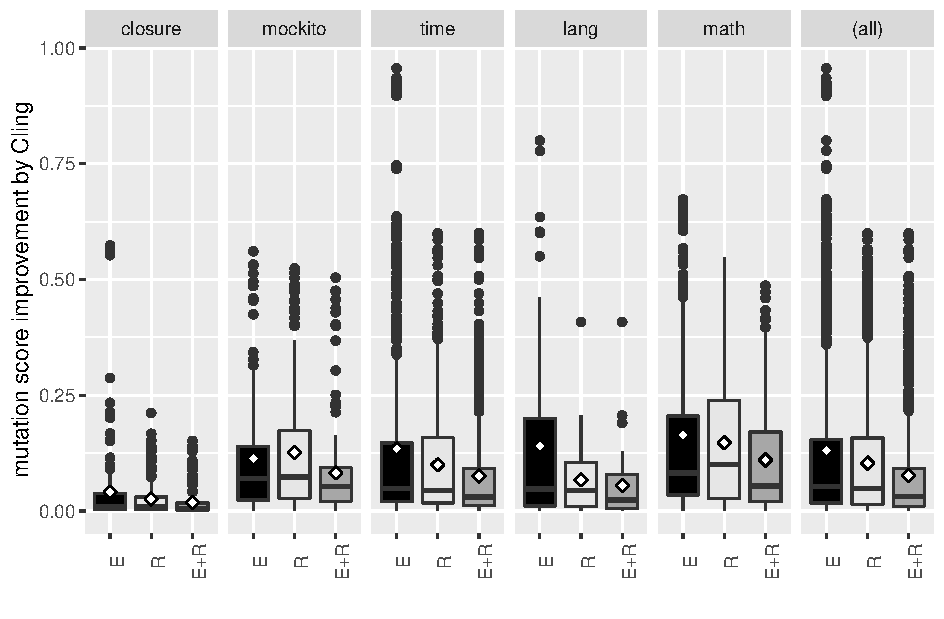
\includegraphics[width=0.75\textwidth]{papers/cling/figures/mutation-diff-boxplot.pdf}
    \caption{Increases in mutation score when combining $T_\integration$ with unit test suites $T_E$, $T_R$ and their union $T_{E+R}$. ($\diamond$) denotes the arithmetic mean and (---) is the median.}
    \label{fig:mutation:diff:boxplot} 
\end{figure}

\begin{table*} [t]
	\center
    \caption{Status (for $T_R$ and $T_E$) of the mutants killed only by $T_{\cling}$. \texttt{Not-covered} denotes the number of mutants killed by $T_{\cling}$, which are not covered by \evosuite test suites, and \texttt{survived} denotes the number of mutants killed by $T_{\cling}$, which are covered by \evosuite tests but not killed.}
	\label{tab:mutant-status-table}
	\resizebox{0.99\textwidth}{!}{%
\begin{tabular}{ l | cc | cc | cc | cc | cc }
\hline 
\textbf{Test Suite}& \multicolumn{2}{c}{\textbf{closure}}& \multicolumn{2}{c}{\textbf{lang}}& \multicolumn{2}{c}{\textbf{math}}& \multicolumn{2}{c}{\textbf{mockito}}& \multicolumn{2}{c}{\textbf{time}} \\ 
 & not-covered & survived & not-covered & survived & not-covered & survived & not-covered & survived & not-covered & survived \\ 
\hline 
$T_E$&  1,988 ( 0.00 )&  881 ( 0.00 )&  3,247 ( 0.01 )&  403 ( 0.00 )&  6,178 ( 0.05 )&  1,747 ( 0.01 )&  5,604 ( 0.04 )&  2,414 ( 0.02 )&  10,905 ( 0.03 )&  5,920 ( 0.01 ) \\ 
$T_R$&  2,480 ( 0.00 )&  780 ( 0.00 )&  2,797 ( 0.01 )&  851 ( 0.00 )&  5,310 ( 0.04 )&  2,558 ( 0.02 )&  4,867 ( 0.04 )&  3,144 ( 0.02 )&  7,431 ( 0.02 )&  9,150 ( 0.02 ) \\ 
\hline 
\end{tabular}
}
\end{table*} 



\begin{table} [t]
	\center
	\caption{Number of mutant killed only only by $T_{\cling}$ and grouped by mutation operators. Integration-level operators are highlighted in \textbf{bold} face.}
	\label{tab:mutant-operators-table}
	\resizebox{0.49\textwidth}{!}{%
\begin{tabular}{ l l | r}
    \hline 
      & \textbf{Mutation operator} & \textbf{\# of kills} \\ 
    \hline 
    1 & \textbf{NonVoidMethodCallMutator} (\textit{RetStaRep}) & 1983 \\ 
    2 & NegateConditionalsMutator & 1638 \\ 
    3 & InlineConstantMutator & 1201 \\ 
    4 & \textbf{ReturnValsMutator} (\textit{RetStaRep}) & 1195 \\ 
    5 & RemoveConditionalMutator\_EQUAL\_IF & 1110 \\ 
    6 & RemoveConditionalMutator\_EQUAL\_ELSE & 1015 \\ 
    7 & \textbf{NullReturnValsMutator} (\textit{RetStaRep}) & 578 \\ 
    8 & \textbf{ArgumentPropagationMutator} (\textit{FunCalDel}) & 518 \\ 
    9 & MathMutator & 513 \\ 
    10 & MemberVariableMutator & 458 \\ 
    11 & \textbf{ConstructorCallMutator} (\textit{FunCalDel}) & 379 \\ 
    12 & RemoveConditionalMutator\_ORDER\_IF & 375 \\ 
    13 & \textbf{VoidMethodCallMutator} (\textit{FunCalDel}) & 374 \\ 
    14 & RemoveConditionalMutator\_ORDER\_ELSE & 348 \\ 
    15 & ConditionalsBoundaryMutator & 322 \\ 
    16 & \textbf{PrimitiveReturnsMutator} (\textit{RetStaRep}) & 309 \\ 
    17 & NakedReceiverMutator & 264 \\ 
    18 & IncrementsMutator & 143 \\ 
    19 & \textbf{BooleanTrueReturnValsMutator} (\textit{RetStaRep}) & 142 \\ 
    20 & RemoveIncrementsMutator & 106 \\ 
    21 & RemoveSwitchMutator & 89 \\
    22 & \textbf{EmptyObjectReturnValsMutator} (\textit{RetStaRep}) & 71 \\ 
    23 & \textbf{BooleanFalseReturnValsMutator} (\textit{RetStaRep}) & 63 \\ 
    24 & InvertNegsMutator & 38 \\ 
    25 & SwitchMutator & 16 \\ 
    \end{tabular}
}
    
\end{table} 

To understand the fault revealing capabilities of \integration, we first show the overall mutation scores in Figure~\ref{fig:mutation:boxplot}.
We show the mutation scores for each subject when mutating class $E$, and apply the test suite $T_E$, $T_R$, and $T_{\integration}$.

As expected, test suites optimized for overall branch (line) coverage ($T_E$), achieve a total higher mutation score (35.3\% on average), simply because a mutant that is on a line that is never executed cannot be killed. 
Thus, $T_E$ scores highest in Figure~\ref{fig:mutation:boxplot}.

Likewise, $T_{\integration}$ scores lower (20.0\% on average), since \integration searches for dedicated interaction pairs, but does not try to optimize overall line coverage.
Note that $T_{\integration}$ achieves the highest mutation score, on average, for classes in \texttt{math}. In contrast, the lowest mutation score is for classes in the complex \texttt{mockito} project.
%
% Finally, the success of \integration is related to the level of CBC achieved for the subject (showed in Figure~\ref{fig:cbccoverage}). A higher CBC helps to exercise a larger amount of different behaviors, which in turn helps to kill mutants. 
% \textcolor{blue}{Annibale: stupid thought: what if we use the correlation test to prove that high CBC does imply a higher mutation score? Otherwise, we cannot claim any relation between the two variables.}

\subsubsection{Combined Analysis}

Figure~\ref{fig:mutation:boxplot} shows that unit test suites $T_E$ and $T_R$ do not kill almost half of the mutants. \integration targets more mutants, including those that remain alive with unit tests.
In Figure \ref{fig:mutation:diff:boxplot}, we report the \emph{increase} in the mutation score when executing $T_\cling$ in addition to $T_E$, $T_R$, and their union $T_{E+R}$.
The main findings are:
\begin{enumerate}
\item On average, 13.01\% of the mutants are killed only by $T_{\integration}$, compared to $T_E$, the unit test suite optimized for the class under test ($E$).
\item This difference decreases to 10.3\%, if we use $T_R$, the unit test suite exercising $E$ via the caller class $R$ (as more class interactions are executed). %This is natural, since both $T_R$ and $T_\integration$ seek to exercise $E$ via $R$.
\item The difference with traditional unit testing is still 7.68\% when comparing \integration with the combined unit test suites $T_{E+R}$, exercising $E$ directly as much as possible as well as indirectly via call sites in $R$.
\end{enumerate}

The outliers in Figure~\ref{fig:mutation:diff:boxplot} are also of interest: for 20 classes (out of 140), \cling was able to generate a test suite where more than half of the mutants were killed \emph{only} by $T_{\cling}$, compared to $T_E$ (i.e., +50\% of mutation score). When compared to $T_{E+R}$, there are four classes for which $T_{\cling}$ kills more than half of the mutants that are killed by neither $T_E$ nor $T_R$. This further emphasizes the complementarity between the unit and integration testing.

%As we can see in this figure, in some classes, more than $50\%$ of the mutants are killed only by $T_{CLING}$ compared to unit-level test suites. In average, the biggest number of extra mutants killed by $T_{CLING}$ is in project Math (about $11 \%$). Also, \integration is less effective in Closure. In average, It increases the number of killed mutants for about $1 \%$.

Table \ref{tab:mutant-status-table} presents the status of the mutants that are killed by $T_{CLING}$ but not by  unit-level test cases. 
What stands out is that many mutants are in fact covered, but not killed by $T_E$ or $T_R$.
Here \cling leverages the context of caller, not only to reach a mutant, but also to \emph{propagate} the (modified) values inside the caller's context, so that the mutants can be eventually killed.


\subsubsection{Mutation Operators}

Moreover, we analyzed the mutation operators that generate mutants that are exclusively killed by $T_{\cling}$. We categorize the mutation operators implemented in PIT into \textit{integration-level} and \textit{non-integration-level}. For this categorization, we rely on the definition of mutation operators for integration testing provided by Delamaro \etal \cite{delamaro2001interface}. 
We observed that ten of the mutation operators implemented in PIT inject integration-level faults. These operators can be mapped to two integration-level operators defined by Delamaro \etal \cite{delamaro2001interface}: \textit{RetStaRep}, which replaces the return value of the called method, and \textit{FunCalDel}, which removes the calls to void method calls and replaces the non-void method calls by a proper value.

Table \ref{tab:mutant-operators-table} lists the number of mutants killed exclusively by $T_{\cling}$ and grouped by mutation operators. Integration-level operators are indicated in bold with the mapping to either \textit{RetStaRep} or \textit{FunCalDel} between parenthesis. As we can see in this table, the most killed mutants are produced by an integration-level operator, and other integration-level operators also produce frequently killed mutants. 
We can see that all of the ten integration-level mutation operators generated mutants that are killable with \integration. 

Furthermore, we can also see that some of the most frequently killed mutants are not produced by integration-level operators. For instance, operator \textit{NegateConditionalsMutator}, which mutates the conditions in the target class, produces the second most frequently killed mutants. These mutants are not killed but also not covered by tests generated by \evosuite.


\begin{figure*}
%   \begin{subfigure}[b]{.5\linewidth}
    \begin{lstlisting}[
        numbers=left,
        firstnumber=1] 
boolean evaluateStepC(StepInterpolator interpolator){
    if (functions.isEmpty()){[...]}
    if (! initialized) {[...]}
    for ([...]) {
        [...];
        // calling the callee class in the next line.
        if (state.evaluateStep(interpolator)){ 
            // Changing variable first
            [...]
        }  
    }
    return first != null;
}
    \end{lstlisting}
    \caption{Method \textit{evaluateStep} in caller class \textit{SwitchingFunctionsHandler}.}
    \label{fig:mutant:example:caller}
%   \end{subfigure}
%   \begin{subfigure}[b]{.5\linewidth}
   
    \begin{lstlisting}[
    numbers=left,
    firstnumber=1] 
boolean evaluateStep(final StepInterpolator interpolator){
[...]    
for([...]){
        if([...]){
            [...];
        }
        if([...]){
            [...];
        }
    }
    [...];
    |return false;|return true; //mutant
}
        \end{lstlisting}
        \caption{Method \textit{evaluateStep} in callee class \textit{switchsState}.}
        \label{fig:mutant:example:callee}
%   \end{subfigure}
%   \caption{Example of a integration-level mutant killed only by \integration From \texttt{Apache commons-math}}
  \label{fig:mutant:example}
\end{figure*}

Lets look at an example of a mutant killed only by \integration. Figure \ref{fig:mutant:example:callee} illustrates one of the mutants in method  \textit{evaluateStep} in class \textit{SwitchState} (callee class) from \textit{Apache commons-math} project. 
This mutant is an integration-level mutation operator (\textit{RetStaRep}) that replaces the boolean return value with the true value.
Method \textit{evaluateStep} in the callee class is called by method \textit{evaluateStepC} (Figure \ref{fig:mutant:example:caller}) in a caller class called \textit{SwitchingFunctionsHandler}. Method \textit{evaluateStepC} must return false if it calls the callee class in a certain situation: (i) the \textit{first} variable in caller class is null, and (ii) callee method returns false because of the execution of line 12 in figure \ref{fig:mutant:example:callee}. 


The generated test suites by \evosuite targeting  \textit{SwitchState} ($T_E$) or class \textit{SwitchingFunctionsHandler} ($T_R$) are both covering this mutant, but they do not kill it. 
$T_E$ easily cover the mutant statement, but it does not have any assertion to check this return value.
Also, $T_R$ covers this statement by calling the right method in \textit{SwitchingFunctionsHandler}. However, as it depicted by figure \ref{fig:mutant:example}, both methods in caller and callee class have multiple branches. So, $T_R$ covers the mutant from another path, which does not reveal the change in the boolean return value.

In contrast, this mutant is killed by the generated test using \integration, targeting \textit{SwitchingFunctionsHandler} and \textit{SwitchState} as the caller and callee classes, respectively (Listing \ref{list:clingTest}).
According to the assertion in line 5 of this test case, \textit{switchingFunctionsHandler0.evaluateStep} must return false. However, the mutant changes the returned value in line 7 of the caller class (Figure \ref{fig:mutant:example:caller}), and thereby the true branch of the condition in line 7 is executed. This true branch changes the value of variable \textit{first} from null to a non-null value. Hence, the \textit{evaluateStep} method in the caller class returns true in line 12. So, the assertion in the last line of Listing \ref{list:clingTest} kills this mutant.

\begin{lstlisting}[frame=tb,
    caption={\cling test case killing mutant in Figure~\ref{fig:mutant:example}},
    label=list:clingTest,
    captionpos=t,
    numbers=left,
    float=t,
    belowskip=-2.5em,
    firstnumber=1]
    public void test07()  throws Throwable  {
        [...]
        boolean boolean1 = switchingFunctionsHandler0.evaluateStepC(stepInterpolator0);
        assertTrue(boolean1 == boolean0);
        assertFalse(boolean1);
    }
    
\end{lstlisting}
\subsubsection{Summary}

The test suite generated by \cling for a caller $R$ and callee $E$, can kill \emph{different} mutants than unit test suites for $E$, $R$ or their union, increasing the mutation score on average with 13.09\%, 10.04\%, and 7.71\%, respectively, with outliers well above 50\%.
Our analysis indicates that many of the most frequently killed mutants are produced by integration-level mutation operators.

\subsection{Integration Faults Exposed by \integration (RQ3)}

\begin{lstlisting}[frame=tb,
    caption={Exception captured only by \integration in Closure},
    label=list:divzero,
    captionpos=t,
    numbers=left,
    float=t,
    belowskip=-2.5em,
    firstnumber=1]
    java.lang.NullPointerException
    com.google.javascript.rhino.head.Decompiler.appendString(Decompiler.java:226)
    com.google.javascript.rhino.head.Decompiler.addName(Decompiler.java:156)
    com.google.javascript.rhino.head.IRFactory.transformName(IRFactory.java:833)
    com.google.javascript.rhino.head.IRFactory.transform(IRFactory.java:157)
\end{lstlisting}

\begin{lstlisting}[frame=tb,
    caption={\cling test case triggering the crash in Listing~\ref{list:divzero}},
    label=list:testdivzero,
    language=java,
    captionpos=t,
    numbers=left,
    float=t,
    belowskip=-2.5em,
    firstnumber=1]
public void testFraction() {
    IRFactory iRFactory0 = new IRFactory();
    Name name0 = new Name(65536, 65536);

    // Undeclared exception!
    iRFactory0.transform(name0);
}
\end{lstlisting}

In our experiments, \integration generates 51 test cases that triggered an unexpected exception in one of the subject systems. 
None of those unexpected exceptions were observed during the execution of the test cases generated by \evosuite.
%These remained undetected by any of the corresponding test cases generated by the $40$ executions of \evosuite (20 for each caller, and 20 for each callee class, for the pairs tested by \integration).

We performed a manual root cause analysis for all 51 unexpected exceptions to check if they are stemming from a real integration-level fault. For this analysis, we check the API documentation to see if the generated test cases break any precondition. We indicated a test case as a bug revealing test if it does not violate any precondition according to the documentation, and it truly exposes an issue about the interaction between the caller and callee class. According to our manual analysis, of the 51 test cases generated by \cling, 32 are \textbf{bug revealing}.

%
% Of the 29 crash-inducing test cases, 21 were found in \textit{Closure}, four in \textit{Time}, and another four in \textit{Math}.
% For six of the 29 integrations tested, the caller and callee belonged to the same class hierarchy (shared a superclass other than Object).

To illustrate the type of problem detected by \integration, consider the test case it has generated in Listing~\ref{list:testdivzero} and the induced stack trace (for a \texttt{NullPointerException}) in Listing~\ref{list:divzero}.
% These are from the Closure Compiler \texttt{Fraction} class, which can be used to represent fractions like $1/3$ or $3/4$. There are several ways to \emph{format} fractions, represented by the \texttt{FractionFormat} class, and its subclass \texttt{Proper\-Fraction\-Format}.

This test aims to invoke a method, called \texttt{transform}, in class \texttt{IRFactory} from the Closure Compiler. This method needs an object from another class, called \texttt{Name}, as an input parameter. This class has various constructors, in which multiple local variables are set. One of these local variables is a String named \texttt{identifier}. Most of the constructors in class \texttt{Name} sets a value for this String. However, one of the specific constructors (\texttt{Name(int pos, int len)}) keeps the value of \texttt{identifier} to null. The generated test by \cling uses this specific constructor to instantiate an object from \texttt{Name} and passes this object to method \texttt{transform}. This method gets \texttt{identifier} by calling the getter method in \texttt{Name} and passes it to another class (\texttt{Decompiler}) without checking it. 
Finally a method in \texttt{Decompiler}, called \texttt{appendString}, uses this passed \texttt{null} String without checking it and it leads to a \texttt{NullPointerException}. We do note that the documentation available in the involved classes does not limit the occurrence of this scenario.

In this particular example, a constructor in class \texttt{Name} assumes that having a null value for \texttt{identifier} is not a problem. In contrast, class \texttt{IRFactory} assumes that this variable can never be null and passes it as a proper String to another class to use it.
The \integration integration testing approach brought these conflicting assumptions together, triggering the stack trace of Listing~\ref{list:divzero}.
% The various classes and methods involved in fractions make assumptions about denominators being zero or not; one class assumed an invariant that the denominator can never be zero. This was indeed ensured by most constructors, but unfortunately not by all.



%
% The test case obtained by \integration implicitly creates a fraction by parsing an empty string. Under the hood this leads to the creation of a fraction from \texttt{Double.NaN}. Fractions can be created from any double, and the \texttt{Fraction} class then finds the corresponding minimal nominator and denominator (e.g., 3 and 4 for 0.75). For \texttt{Double.NaN} this approximation leads to a denominator that is zero.
% At the same time, the \texttt{format} method seeks to display the fraction value, and therefore computes the actual division, triggering the failure.

As is typical for integration faults, this problem can be fixed in multiple ways. The most consistent would be to adjust the \texttt{transform} method in class \texttt{IRFactory}, to check the value of \texttt{identifier} in the passed \texttt{Name} object. This then would ensure that it does not use a null value for calling methods in \texttt{Decompiler}.


The detailed version of the performed manual analysis for all of the 51 exceptions are openly available\footnote{\url{https://github.com/STAMP-project/Cling-application/tree/master/data\_analysis/manual-analysis}}.

\subsubsection{Summary}
\integration-based automated testing of $\langle$caller, callee$\rangle$ class pairs exposes actual problems that are not found by unit testing either the caller or callee class individually. These problems relate to conflicting assumptions on the safe use of methods across classes.